\chapter[Implied volatility estimation for European options in jump-diffusion dynamics]{Implied volatility estimation for European options in jump-diffusion dynamics}
\chaptermark{Implied volatility -- European options with jumps}

\section{A PIDE analogue of Dupire's equation}
In this section, we will derive a PIDE that is the analogue of Dupire's equation as seen in \cite{Gatheral2006}. The Dupire-like PIDE will serve as the platform for computing the implied volatility of options with jump-diffusion asset dynamics.

\subsection{Homogeneity of the solution}
First, we assume that the payoff function $\phi$ now depends on a parameter~$x' > 0$ (i.e., $\phi = \phi(x;x')$).  The motivation for this is that in the case of a European put or call, $x'$ represents the strike price. Furthermore, we assume that $\phi$ is homogeneous of degree one in~$x$ and $x'$. \textcolor{blue}{That is, we assume
$$
	\phi(\beta x; \beta x') = \beta \phi(x;x').
$$}
Note that standard put and call payoffs satisfy this assumption. We show that the option price function~$v$ is homogeneous of degree one in~$x$ and $x'$. That is, we want to show for $v = v(x,t; x')$ that
		\begin{equation}
			\label{eqn:homogen}
			v(\beta x, t; \beta x') = \beta v(x,t; x')
		\end{equation}
for all $\beta > 0$. This equality can be proven via a uniqueness argument as follows. We first express \eqref{eqn:PIDE} as $\mathscr{L} v = 0$. Now let $w = w(x,t; x')$ solve the following final value problem:
		\begin{align}
			\label{eqn:subPIDE}
			\begin{split}
			&\mathscr{L}w = 0, \qquad w(x,T; x') = \beta\phi(x;x').
			\end{split}
		\end{align}
Next, we define the function $v_1(x,t;x') = \beta v(x,t;x')$, where $v$ is a solution to (\ref{eqn:PIDE}), (\ref{eqn:PIDEcondition}). Then
	\begin{align*}
		\mathscr{L}v_1 = \beta \mathscr{L}v = 0.
	\end{align*}
For the terminal condition, since $v(x,T;x') = \phi(x;x')$, this implies that
	\begin{equation*}
		v_1(x,T;x') = \beta v(x,T; x') = \beta\phi(x;x').
	\end{equation*}
Therefore $v_1$ satisfies the final value problem \eqref{eqn:subPIDE}. On the other hand, we now let $v_2(x,t,x') = v(\beta x, t; \beta x')$. Computing the derivatives gives
	\begin{equation*}
		\fr{\pr v_2}{\pr x} = \beta D_1v, \quad \fr{\pr^2 v_2}{\pr x^2} = \beta^2 D_{11}v,
	\end{equation*}
where $D_1$ and $D_{11}$ represent the first and second partial derivatives with respect to the first argument, respectively. Substituting these into (\ref{eqn:subPIDE}), we get
	\begin{align*}
		\mathscr{L}v_2 = \mathscr{L}v = 0,
	\end{align*}
and by the homogeneity of $\phi$, the terminal condition is
	\begin{align*}
		v_2(x,T;x') = v\left( \beta x, T; \beta x' \right) = \phi(\beta x; \beta x') = \beta \phi(x;x').
	\end{align*}
Hence $v_2$ also satisfies the final value problem \eqref{eqn:subPIDE}. By uniqueness, we have
	\begin{equation*}
		v\left(\beta x, t; \beta x'\right) = v_2(x,t;x') = v_1(x,t;x') = \beta v(x,t;x'),
	\end{equation*}
thus proving the homogeneity property for $v$ and any general payoff $\phi$ that is homogeneous of degree one in~$x$ and $x'$.

\subsection{Derivation of a Dupire-like PIDE via Euler's theorem on homogeneous functions}
The partial derivatives of the Dupire equation~\cite{Gatheral2006} are with respect to the strike price $K$. Thus to derive a Dupire-like PIDE, we will require partial derivatives in terms of $x'$ (the analogous variable for $K$). This can be done by invoking Euler's theorem for homogeneous functions~\cite[pp. 317]{Kishan2007} to $v$ and we get
	\begin{equation*}
		x\fr{\pr v}{\pr x} + x'\fr{\pr v}{\pr x'} = v,
	\end{equation*}
since $v$ has been shown to be homogeneous in $x$ and $x'$ of degree one. By differentiating the above equation with respect to $x$ and $x'$, we obtain
	\begin{equation*}
		x\fr{\pr^2 v}{\pr x^2} = -x'\fr{\pr^2 v}{\pr x \pr x'}, \quad x'\fr{\pr^2 v}{\pr x'^2} = -x\fr{\pr^2 v}{\pr x' \pr x},
	\end{equation*}
respectively. Hence it follows that
	\begin{equation*}
		x^2\fr{\pr^2 v}{\pr x^2} = x'^2\fr{\pr^2 v}{\pr x'^2}.
	\end{equation*}
The only term left to account for is the integral in (\ref{eqn:PIDE}). Notice that the first integrand term depends on~$y$; we want to transfer the dependency on $y$ to the third argument (i.e., $x'$). This can be achieved by the homogeneity property in (\ref{eqn:homogen}), and we obtain
	\begin{align*}
		v(xy,t; x') &= v\left(xy,t;\fr{x'y}{y}\right) = yv\left( x,t;\fr{x'}{y} \right).
	\end{align*}
Thus, setting $u(x',t; x) = v(x,t; x')$ and replacing all the $x$ derivatives with $x'$ derivatives and substituting the above rearrangement for the integrand, we get
	\begin{align}
		\label{eqn:DupireLike}
		\begin{split}
		\fr{\pr u}{\pr t} &- (q(t) + \kappa\lambda)u - (r(t) - q(t) - \kappa\lambda)x'\fr{\pr u}{\pr x'} + \fr{1}{2}\sigma(t)^2x'^2\fr{\pr^2 u}{\pr x'^2} \\
		& {} + \lambda \int_0^\infty \left( yu\left( \fr{x'}{y},t; x \right) - u(x',t; x) \right)f(y) \, \d y = 0
		\end{split}
	\end{align}
with
	\begin{equation}
		\label{eqn:DupireCond}
		u(x',T; x) = \phi(x';x),
	\end{equation}
since $u$ now depends on the variables $x'$ and $t$ with $x$ as a parameter. Equations~(\ref{eqn:DupireLike}) and (\ref{eqn:DupireCond}) together form the Dupire-like PIDE system for options in a jump-diffusion framework. Note that this reduces to the standard Dupire PDE as seen in \cite{Gatheral2006} in the absence of jumps (i.e., $\lambda = 0$) when $\phi$ is either the call or put payoff.

\section{Implied volatility formula}
From (\ref{eqn:DupireLike}) and (\ref{eqn:DupireCond}), it is possible to now solve the inverse problem of implied volatility estimation. Throughout the remainder of this section, we will assume that~$r$ and $q$ are constants. Suppose that we are given $u(x',0;S_0)$ for all $x' > 0$. We wish to derive an explicit formula for $\sigma$ in terms of certain integrals of $u$ with respect to $x'$. The reason for this is that in practice one can observe different time-zero option prices~$u_1,\, u_2, \, \ldots, u_m$ for varying strike prices~$K_1, \, K_2, \, \ldots, K_m$, here corresponding to different values of $x'$. Once we can extrapolate $u$ for extreme values of $x'$, we would know the entire time-zero profile of $u$.

First, denote by $\hat u$ the Mellin transform of $u$ with respect to $x'$, i.e.,
	\begin{equation*}
		\hat u(\xi,t) = \int_0^\infty (x')^{\xi-1} u(x',t; x) \, \d x'.
	\end{equation*}
We take the Mellin transform of (\ref{eqn:DupireLike}) and (\ref{eqn:DupireCond}) with respect to $x'$ to obtain
	\begin{align}
		\label{eqn:mellinDUPIRE}
		\begin{split}
			\fr{\pr \hat u}{\pr t} - G_{\lambda}(\xi)\hat u(\xi,t) = 0, \quad \hat u(\xi,T) = \hat \phi(\xi),
		\end{split}
	\end{align}
where
	\begin{equation}
		G_{\lambda}(\xi) = -\left( \fr{\sigma^2}{2}\xi(\xi+1) + (r - q - \kappa\lambda)\xi - (	q + \kappa\lambda) + \lambda\E[Y^{\xi+1} - 1] \right).
	\end{equation}
We are left with an ODE in $t$. Solving (\ref{eqn:mellinDUPIRE}) gives
	\begin{equation}
		\label{eqn:mellinDUPIREode}
		\hat u(\xi,t) = e^{-G_{\lambda}(\xi)(T-t)}\hat \phi(\xi).
	\end{equation}
We can proceed to isolate $\sigma^2$ in (\ref{eqn:mellinDUPIREode}) to yield
	\begin{align}
		\label{eqn:sigmaMellin}
		\begin{split}
		\sigma^2 &= \fr{2}{\xi(\xi+1)}\bigg( \fr{\ln( \hat u(\xi,t)/\hat\phi(\xi) )}{T-t} - (r-q-\kappa\lambda)\xi + (q+\kappa\lambda) - \lambda\E[Y^{\xi+1} - 1] \bigg),
		\end{split}
	\end{align}
where we have the flexibility to choose a value of $\xi$. Theoretically, $\sigma^2$ should be constant for any value of $\xi$ and $t$, provided the Mellin transform of $u$ exists. Furthermore, it should be emphasised that (\ref{eqn:sigmaMellin}) can be applied to any type of payoff and jump. When $\lambda = 0$, \eqref{eqn:sigmaMellin} gives an explicit formula for the implied volatility in the usual diffusion framework.

\section{Numerical simulations}
\label{sec:numerics}
This section will contain the numerical results obtained from the implied volatility formula (\ref{eqn:sigmaMellin}) for lognormal jumps. To test the validity of the model, we will require an initial $\sigma$ value to generate option prices before solving the inverse problem. The results will be divided into two sets: the first set will be implementing purely theoretical data; the second set will be generated using pseudo-market data that attempts to mimic observed market prices and values. We will now elaborate on how the option prices are obtained. For definiteness, we will consider a time-zero European call where the underlying follows standard diffusion dynamics (i.e., no jumps). That is, in \eqref{eqn:EUcall} we set $t = 0$, $x = S_0$, assume $r$, $q$, and $\sigma$ are constant, and view this as a function of $K$ given as
	\begin{equation}
		\label{eqn:EUcallK}
		v^{\text{call}}(K) = S_0e^{-qT}N\left( z_1\left( \fr{S_0}{K}, 0, T \right) \right) - Ke^{-rT}N\left( z_2\left( \fr{S_0}{K}, 0, T \right) \right),
	\end{equation}
where $z_1$ and $z_2$ are defined as they are in \eqref{eqn:z1} and \eqref{eqn:z2}, respectively.

\subsection{Theoretical data for option prices}
The Mellin transform is valid in the domain $[0,\infty)$. Since this implied volatility scheme incorporates a Mellin transform with respect to the strike price~$K = x'$ for a fixed~$x = S_0$, we require time-zero option prices for varying $K \in [0,\infty)$. Numerically, we will use discrete 200 values of $K \in [1.0\times10^{-6},8S_0]$ evenly spaced to simulate continuity for the entire domain $K > 0$. This will yield 200 call prices.  In practice, this is seldom applicable as many sources for financial data will only list discrete option prices for a finite set of $K$ values (i.e., much less than 200) and for a fixed asset price~$S_0$. Furthermore, it is often implausible to expect the domain of $K$ to be uniformly spaced. This approach is only included to illustrate the accuracy of the model assuming a very smooth dataset.

\subsection{Pseudo-market data for option prices}
As mentioned before, the finite number of discrete option prices may prove insufficient in exhibiting a continuous behaviour in the option price profile. Hence we require a method for approximating the data beyond the option prices provided. The following procedure will be demonstrated for a call option in the absence of jumps to simplify the calculations. However, these steps can be adapted when accounting for jumps in the asset dynamics.

We assume that we have a set of call prices~$v_1 > v_2 > \cdots > v_{m - 1} > v_m$ with corresponding strike prices~$K_1 < K_2 < \cdots < K_{m - 1} < K_m$. It is known from \cite{Bowling2009} that the best one-parameter logistic approximation of the standard normal CDF $N$ for all $z \in \R$ is given by
	\begin{equation*}
		N(z) \approx \frac{1}{1 + e^{-a z}}, \quad a = 1.702,
	\end{equation*}
where the maximum difference between the approximation and exact expression for $N$ is less than $0.001$ for $z \in [-4.5,4.5]$. %Check what happens outside -4.5 and 4.5
Now for $z < 0$ we have
	\begin{equation*}
		N(z) \approx \fr{e^{az}}{1+e^{az}} = e^{az}(1-e^{az}+e^{2az}-\cdots) = e^{az} - e^{2az} + e^{3az} - \cdots.
	\end{equation*}
Hence we can take $N(z) \approx e^{az}$ for $z \ll -1$. Using this logistic estimation in \eqref{eqn:EUcallK}, this approximates to
	\begin{equation*}
		v^{\text{call}}(K) \approx \frac{S_0 e^{-q T}}{1 + e^{-a d_1(S_0/K,0,T)}} - \frac{K e^{-r T}}{1 + e^		{-a d_2(S_0/K,0,T)}} = \frac{S_0 e^{-q T}}{1 + e^{-a d_1}} - \frac{K e^{-r T}}{1 + e^		{-a d_2}},
	\end{equation*}
where $d_1$ and $d_2$ are defined as
	\begin{equation*}
		d_1 = z_1\left( \fr{S_0}{K},0,T \right), \quad d_2 = z_2\left( \fr{S_0}{K}, 0, T\right)
	\end{equation*}
using \eqref{eqn:z1} and \eqref{eqn:z2}, respectively under the assumption of constant parameters.
When $|K| \ll 1$ we see that $d_1 \gg 1$ and $d_2 \gg 1$; hence $v^{\text{call}}(K) \approx S_0 e^{-q T} - K e^{-r T}$. Therefore we assume that
	\begin{equation*}
		v^{\text{call}}(K) = S_0e^{-qT} - \beta K, \quad 0 < K \le K_1
	\end{equation*}
for some $\beta > 0$. Using $K_1$ to extrapolate, we see from $v^{\text{call}}(K_1) = v_1$ that we obtain
%Therefore we assume that
%\begin{equation*}
%\Vcall(K) = \kappa - \beta K, \quad 0 < K \le K_2
%\end{equation*}
%for some $\kappa, \beta > 0$. From $\Vcall(K_1) = V_1$ and $\Vcall(K_2) = V_2$ we obtain
	\begin{equation*}
		\beta = \fr{S_0e^{-qT} - v_1}{K_1}.
	\end{equation*}
Conversely, when $K \gg 0$ we have $-d_1 \gg 1$ and $-d_2 \gg 1$. Using $N(z) \approx e^{az}$ for $-z \gg 1$, we can simplify $N(d_1)$ and $N(d_2)$ and approximate \eqref{eqn:EUcallK} by
	\begin{equation*}
		v^{\text{call}}(K) \approx S_0 e^{-q T} e^{a d_1} - K e^{-r T} e^{a d_2}.
	\end{equation*}
As $d_1 = d_2 + \sigma \sqrt{T}$,
	\begin{equation*}
		e^{a d_2} = e^{a\left(\log(S_0/K) + (r - q - \sigma^2/2) T\right)/\left(\sigma \sqrt{T}\right)} = \left(\frac{S_0}{K}\right)^{a/\left(\sigma \sqrt{T}\right)} e^{a(r - q - \sigma^2/2) \sqrt{T}/\sigma}.
	\end{equation*}
Similarly,
	\begin{equation*}
		e^{a d_1} = e^{a \sigma \sqrt{T}} e^{a d_2},
	\end{equation*}
hence we have
	\begin{equation*}
		v^{\text{call}}(K) \approx \left(S_0 e^{-q T} e^{a \sigma \sqrt{T}} - K e^{-r T}\right) \left(\frac			{S_0}{K}\right)^{a/\left(\sigma \sqrt{T}\right)} e^{a (r - q - \sigma^2/2) \sqrt{T}/\sigma}.
	\end{equation*}
Therefore we assume that
	\begin{equation*}
		v^{\text{call}}(K) = \frac{\gamma_1}{K^\delta} + \frac{\gamma_2}{K^{\delta-1}}, \quad K \ge K_{m}
	\end{equation*}
for some $\gamma_1,\gamma_2, \delta > 0$. We will need to use $K_{m-1}$ and $K_{m}$ to extrapolate, but we also require another data point. For the call option, $v^{\text{call}}(K) \rightarrow 0$ as $K \rightarrow \infty$, thus we let $K_L \gg K_m$ represent the strike price ``near'' infinity. We see from $v^{\text{call}}(K_{m - 1}) = v_{m - 1}$, $v^{\text{call}}(K_m) = v_m$, and $v^{\text{call}}(K_L) \approx 0$, and we deduce that
	\begin{align*}
		&\delta = \fr{\log\left( v_{m-1}/v_m\right) + \log\left((K_L - K_m)/(K_L-K_{m-1}) \right)}{\log(K_{m}/K_{m-1})}, \\
		&\gamma_2 = \frac{v_mK_m^\delta}{K_m - K_L}, \quad
		\gamma_1 = -K_L \gamma_2, \quad K_L \gg K_m.
	\end{align*}
Thus the call option function can be reformulated to become
	\begin{equation}
		\label{call-interpolate}
		v^\text{call}(K) =
			\begin{cases}
				S_0e^{-qT} - \beta K & 0 < K \le K_1,\\
				v_j & K = K_j, \enskip j = 1,\ldots,m,\\
				\frac{\gamma_1}{K^\delta} + \frac{\gamma_2}{K^{\delta-1}} & K \ge K_{m},
			\end{cases}
	\end{equation}
where $v_1,\ldots,v_m$ are the observed call prices. A similar process can also be adopted for the European call or put with jumps. Figures~\ref{fig:euro-call-bs} and~\ref{fig:euro-call-extrapolate} show the profile for the call option with both theoretical and pseudo-market data, respectively.

\begin{figure}[!h]
		\centering
		\subfigure[Call prices computed using \eqref{eqn:EUcallK} with $200$ equally spaced nodes for $K$ between $10^{-6}$ and $8S_0$. \label{fig:euro-call-bs}]{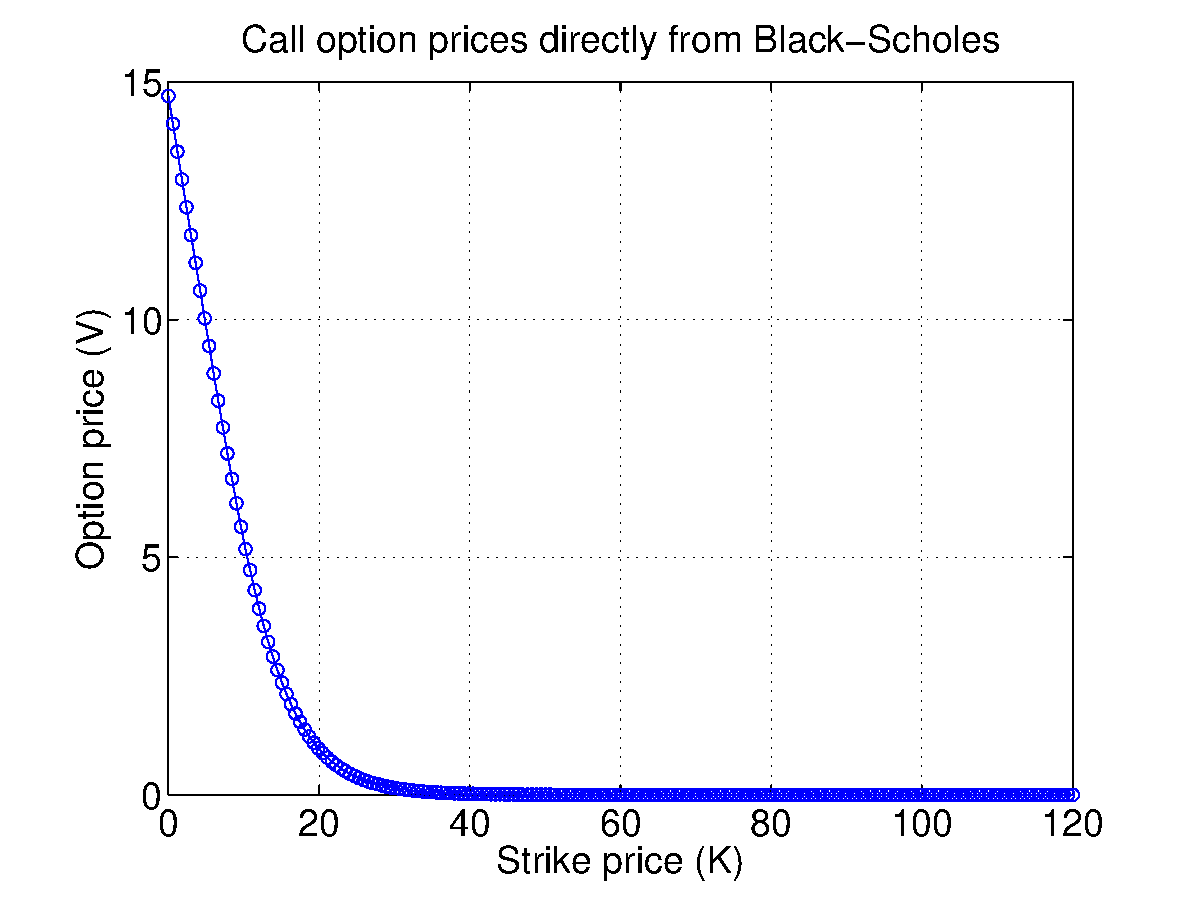
\includegraphics[width=0.49\linewidth]{figures/call-bs-prices.eps}\hspace*{3pt}}
		\subfigure[Call prices computed using \eqref{eqn:EUcallK} for pseudo-observed Black-Scholes values and \eqref{call-interpolate} to extrapolate. \label{fig:euro-call-extrapolate}]{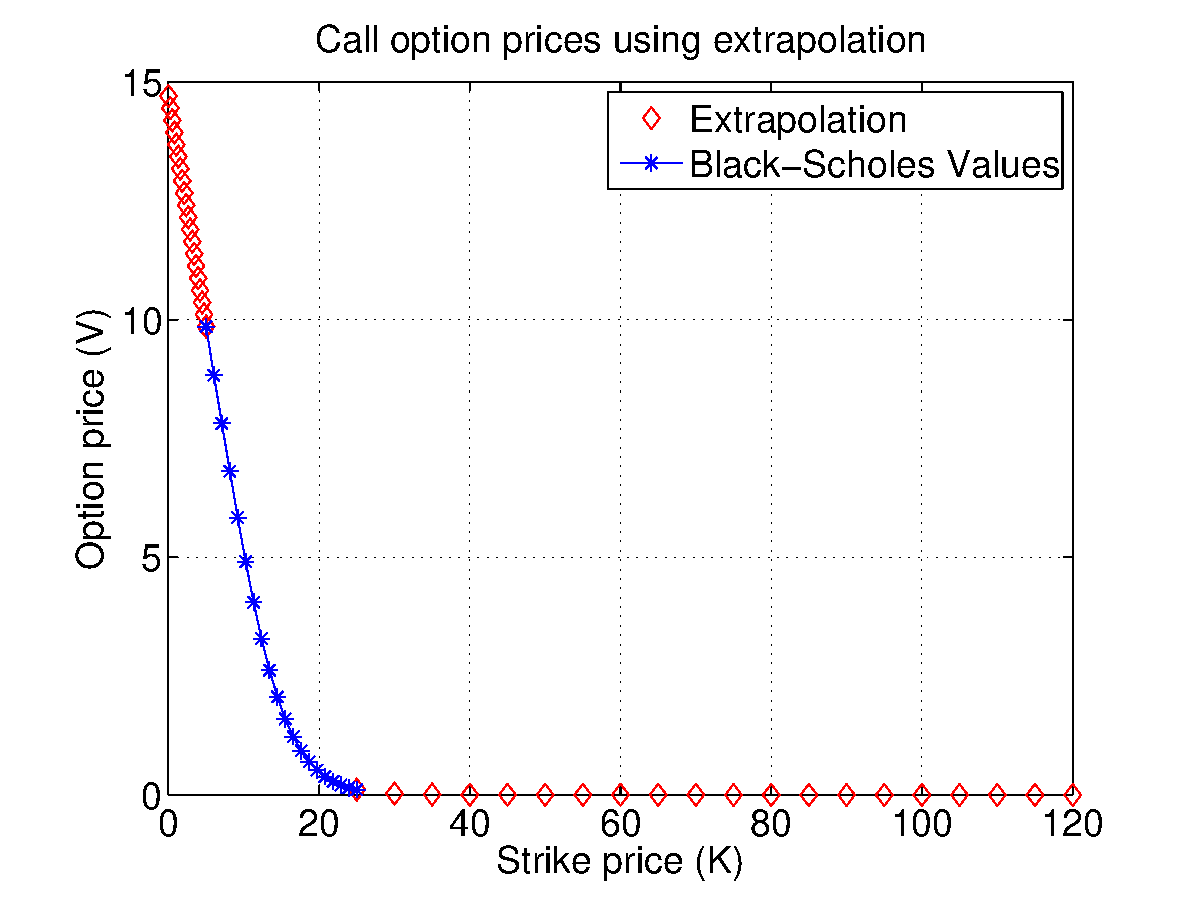
\includegraphics[width=0.49\linewidth]{figures/call-extrapolate-prices.eps}
			}
		\caption{Call option profiles for $K > 0$. The parameter values are $S_0 = 15$, $T = 0.3$, $r = 0.03$, $q=0.02$, and $\sigma = 0.3$.}
\end{figure}


\subsection{Algorithm}
The algorithm for computing $\sigma^2$ for a call option is as follows:
	\begin{enumerate}
		\item Obtain option data~$v_1, v_2,  \cdots,  v_m$~ for ~$K_1 < K_2 < \cdots < K_m$ either using theoretical, pseudo-market or actual market data.
			\begin{enumerate}
				\item Theoretical data -- use (\ref{eqn:EUcallK}) or (\ref{eqn:mertonSoln}) (with appropriate adjustments to the notation) and ensure ~$K_1, K_2, \hdots, K_m$ are 200 evenly spaced nodes between $10^{-6}$ and $8S_0$ (adjust if $8S_0 < K_m$).
				\item Pseudo-real or market data -- generate $v_1, v_2, \cdots, v_m$ using theoretical data or observed from the market, then use \eqref{call-interpolate} (adapt for jumps if necessary) to create more data points for a smoother profile. For $K \approx 0$, use $1.0\times10^{-6}$; for $K \gg 0$, use $8S_0$ (adjust if $8S_0 < K_m$).
			\end{enumerate}
		\item Choose a value of $\xi$.
		\item Evaluate $\hat v^\text{call}(\xi) = \int_0^\infty K^{\xi - 1} v^\text{call}(K) \, \d K$ via numerical integration (e.g., Gauss-Lobatto or Gauss-Kronrod quadrature), where $v^\text{call}$ is the entire time-zero option profile.
		\item Substitute the value for $\hat v^\text{call}(\xi)$ into \eqref{eqn:sigmaMellin} and compute $\sigma^2$.
	\end{enumerate}


\subsection{Results}

We will now report the implied volatility estimations for both theoretical option data and pseudo-market option prices via extrapolation. The parameter values used are $S_0 = 15$, $r = 0.05$, $q = 0.03$, and $T = 0.025$. We used $\sigma = 0.15$ and $\sigma = 0.3$ as initial seeds to generate the corresponding option prices. All simulations are performed in MATLAB using a European call option (with and without jumps). The Mellin transform is computed using the adaptive Gauss-Kronrod quadrature scheme available in MATLAB. The MATLAB code is provided in Appendix C.2.

\subsubsection{Theoretical data}
For the theoretical data, \eqref{eqn:optionLN} is used to generate 200 European call option prices with lognormal jumps for $K \in [1.0\times 10^{-6}, 8S_0]$. The associated lognormal parameters are chosen to be $\lambda = 0.10$, $\mu_Y = -0.90$, and $\sigma_Y = 0.45$. We generated 30 terms from the infinite series. To illustrate the consistency of the algorithm, several $\xi$ values are selected for the Mellin transform. The domain chosen is $\xi \in [1.0,5.0]$ in discrete increments of 0.25.
Tables~\ref{tab:sig015Theo} and \ref{tab:sig030Theo} show the numerical approximations for $\sigma$ against the true values.

\begin{table}\small{
\parbox{.45\linewidth}{
\centering
\begin{tabular}{ |c|c|c| }
\hline
\multicolumn{3}{ |c| }{\textbf{Implied volatility estimation for $\sigma = 0.15$}} \\
\multicolumn{3}{ |c| }{Avg. CPU time: 0.1 s}\\
\hline
$\xi$ & Estimated $\sigma$ & Absolute error \\ \hline
1.0 & 0.150001657453424 & $1.6 \times 10^{-6}$ \\
1.25 & 0.149999916945745 & $8.3 \times 10^{-8}$ \\
1.5 & 0.150004007140589 & $4.0 \times 10^{-6}$ \\
1.75 & 0.150000231848765 & $ 2.3 \times 10^{-7}$ \\
2.0 & 0.150000372512579 & $3.7 \times 10^{-7}$ \\
2.25 & 0.150000519892163 & $5.1 \times 10^{-7} $ \\
2.5 & 0.150000665164591& $6.6 \times 10^{-7}$ \\
2.75 & 0.150000808303685 & $ 8.0 \times 10^{-7} $ \\
3.0 & 0.150000949189142 & $ 9.4 \times 10^{-7} $ \\
3.25 & 0.150001087644665 & $1.0 \times 10^{-6}$ \\
3.5 & 0.150001223391692 & $ 1.2 \times 10^{-6} $ \\
3.75 & 0.150001355979046 & $ 1.3 \times 10^{-6}$ \\
4.0 & 0.150001484661131 & $ 1.4 \times 10^{-6}$ \\
4.25 & 0.150001608185628 & $1.6 \times 10^{-6}$ \\
4.5 & 0.150001724425047 & $ 1.7 \times 10^{-6}$ \\
4.75 & 0.150001829737164 & $1.8 \times 10^{-6}$ \\
5.0 & 0.150001917853050 & $1.9 \times 10^{-6}$ \\
\hline
\end{tabular}
\caption{Implied volatility estimations and errors for different $\xi$ when $\sigma = 0.15$ using pure theoretical option data from \eqref{eqn:optionLN}. Average CPU time is given in seconds.}
\label{tab:sig015Theo}
}
\hfill
\parbox{.45\linewidth}{
\centering
\begin{tabular}{ |c|c|c| }
\hline
\multicolumn{3}{ |c| }{\textbf{Implied volatility estimation for $\sigma = 0.3$}} \\
\multicolumn{3}{ |c| }{Avg. CPU time: 0.1 s}\\
\hline
$\xi$ & Estimated $\sigma$ & Absolute error \\ \hline
1.0 & 0.300000812537166 & $8.1 \times 10^{-7}$ \\
1.25 & 0.300000602264498 & $6.0 \times 10^{-7}$ \\
1.5 & 0.300001642090901 & $1.6 \times 10^{-6}$ \\
1.75 & 0.300000647148822 & $ 6.4 \times 10^{-7}$ \\
2.0 & 0.300000660419985 & $6.6 \times 10^{-7}$ \\
2.25 & 0.300000671406796 & $6.7 \times 10^{-7} $ \\
2.5 & 0.300000680367558 & $6.8 \times 10^{-7}$ \\
2.75 & 0.300000687348957 & $ 6.8 \times 10^{-7} $ \\
3.0 & 0.300000692310426 & $ 6.9 \times 10^{-7} $ \\
3.25 & 0.300000695116983 & $6.9 \times 10^{-7}$ \\
3.5 & 0.300000695475283 & $ 6.9 \times 10^{-7} $ \\
3.75 & 0.300000692830239 & $ 6.9 \times 10^{-7}$ \\
4.0 & 0.300000686190937 & $ 6.8 \times 10^{-7}$ \\
4.25 & 0.300000329275066 & $3.2 \times 10^{-7}$ \\
4.5 & 0.300000337379160 & $ 3.3 \times 10^{-7}$ \\
4.75 & 0.300000329776874 & $3.2 \times 10^{-7}$ \\
5.0 & 0.300000298131713 & $2.9 \times 10^{-7}$ \\
\hline
\end{tabular}
\caption{Implied volatility estimations and errors for different $\xi$ when $\sigma = 0.3$ using pure theoretical option data from \eqref{eqn:optionLN}. Average CPU time is given in seconds.}
\label{tab:sig030Theo}
}}
\end{table}

\begin{table}\small
\parbox{.45\linewidth}{
\centering
\begin{tabular}{ |c|c|c| }
\hline
\multicolumn{3}{ |c| }{\textbf{Implied volatility estimation for $\sigma = 0.15$}} \\
\multicolumn{3}{ |c| }{Avg. CPU time: 0.002 s}\\
\hline
$\xi$ & Estimated $\sigma$ & Absolute error \\ \hline
1.0 & 0.149998728439811 & $1.2 \times 10^{-6}$ \\
1.25 & 0.150027834813882 & $2.7 \times 10^{-5}$ \\
1.5 & 0.150054557535829 & $5.4 \times 10^{-5}$ \\
1.75 & 0.150080609531067 & $ 8.0 \times 10^{-5}$ \\
2.0 & 0.150106032110318 & $1.0 \times 10^{-4}$ \\
2.25 & 0.150130843920878 & $1.3 \times 10^{-4} $ \\
2.5 & 0.150155063080464 & $1.5 \times 10^{-4}$ \\
2.75 & 0.150178294968951 & $ 1.7 \times 10^{-4} $ \\
3.0 & 0.150201382384214 & $ 2.0 \times 10^{-4} $ \\
3.25 & 0.150223926634414 & $2.2 \times 10^{-4}$ \\
3.5 & 0.150245946705591 & $ 2.4 \times 10^{-4} $ \\
3.75 & 0.150267456617342 & $ 2.6 \times 10^{-4}$ \\
4.0 & 0.150288471381866 & $ 2.8 \times 10^{-4}$ \\
4.25 & 0.150309005551112 & $3.0 \times 10^{-4}$ \\
4.5 & 0.150329021452815 & $ 3.2 \times 10^{-4}$ \\
4.75 & 0.150348633294877 & $3.4 \times 10^{-4}$ \\
5.0 & 0.150367805351298 & $3.6 \times 10^{-4}$ \\
\hline
\end{tabular}
\caption{Implied volatility estimations and errors for different $\xi$ when $\sigma = 0.15$ using \eqref{eqn:EUcallK} to generate pseudo-market data. Average CPU time is given in seconds.}
\label{tab:sig015Pseudo}
}
\hfill
\parbox{.45\linewidth}{
\centering
\begin{tabular}{ |c|c|c| }
\hline
\multicolumn{3}{ |c| }{\textbf{Implied volatility estimation for $\sigma = 0.3$}} \\
\multicolumn{3}{ |c| }{Avg. CPU time: 0.002 s}\\
\hline
$\xi$ & Estimated $\sigma$ & Absolute error \\ \hline
1.0 & 0.300031895572929 & $3.1 \times 10^{-5}$ \\
1.25 & 0.300045257605552 & $4.5 \times 10^{-5}$ \\
1.5 & 0.300058090390309 & $5.8 \times 10^{-5}$ \\
1.75 & 0.300071242016552 & $ 7.1 \times 10^{-5}$ \\
2.0 & 0.300085040710682 & $8.5 \times 10^{-5}$ \\
2.25 & 0.300099577530501 & $9.9 \times 10^{-5} $ \\
2.5 & 0.300115017586394 & $1.1 \times 10^{-4}$ \\
2.75 & 0.300131558128381 & $ 1.3 \times 10^{-4} $ \\
3.0 & 0.300149410201347& $ 1.4 \times 10^{-4} $ \\
3.25 & 0.300168805884818 & $1.6 \times 10^{-4}$ \\
3.5 & 0.300190000681277 & $ 1.9 \times 10^{-4} $ \\
3.75 & 0.300213193710094 & $ 2.1 \times 10^{-4}$ \\
4.0 & 0.300238860932383 & $ 2.3 \times 10^{-4}$ \\
4.25 &0.300267261118478 & $2.6 \times 10^{-4}$ \\
4.5 & 0.300298771264214 & $ 2.9 \times 10^{-4}$ \\
4.75 & 0.300333806724048 & $3.3 \times 10^{-4}$ \\
5.0 & 0.300372824834949 & $3.7 \times 10^{-4}$ \\
\hline
\end{tabular}
\caption{Implied volatility estimations and errors for different $\xi$ when $\sigma = 0.3$ using \eqref{eqn:EUcallK} to generate pseudo-market data. Average CPU time is given in seconds.}
\label{tab:sig030Pseudo}

}
\end{table}

For the theoretical option prices, the implied volatility estimations for $\sigma = 0.15$ and $\sigma = 0.3$ prove to be quite accurate with errors in the order of $10^{-7}$ to $10^{-6}$. The error remains relatively consistent for all $\xi$ in the allocated domain, which further highlights the precision of the algorithm. It can be argued for $\sigma = 0.15$ that the absolute error is increasing as $\xi$ increases; however, this is primarily linked to approximation errors since the Mellin transform is computed numerically.

\subsubsection{Pseudo-market data}
The pseudo-market option prices are computed using \eqref{eqn:EUcallK} with 20 discrete values of $K \in [5,25]$, and then incorporates \eqref{call-interpolate} to extrapolate and provide continuity to the data.  Although we are considering a scenario with no jumps (i.e., $\lambda = 0$), a similar procedure may be applied in the case of jumps as seen in the previous section using pure theoretical data. Note that the discrete domain for $K$ will need to be adjusted accordingly if $S_0$ changes. Tables \ref{tab:sig015Pseudo} and \ref{tab:sig030Pseudo} list the results for the implied volatility estimation.

Once again, the results are quite satisfactory but the overall absolute error has increased in order of magnitude in comparison to the estimations yielded by the purely theoretical dataset. This is mainly attributed to the extrapolating functions in \eqref{call-interpolate}. Whilst it maintains the monotonicity of the option profile versus the strike price (e.g., monotonically decreasing for a European call against strike), the main source of error lies within the ``tail'' function (i.e., the approximation for the option price as $K \rightarrow \infty$). This will be elaborated upon in the discussion.

\subsubsection{Comparison to other methods}
We will now give a comparison of \eqref{eqn:sigmaMellin} against two other formulas for implied volatility estimation. \textcolor{black}{We first denote $v^\text{call}$ to be observed European call price that is required to compute the implied volatility}. We will use the result by Brenner and Subrahmanyam~\cite{Brenner1988}
	\begin{equation}
		\label{eqn:brensub}
		\sigma \approx \fr{v^\text{call}}{S_0}\sqrt{\fr{2\pi}{T}},
	\end{equation}
Corrado and Miller~\cite{Corrado1996}
	\begin{equation}
		\label{eqn:corrado}
		\sigma \approx \fr{1}{S_0 + K}\sqrt{\fr{2\pi}{T}}\left( v^\text{call} - \fr{S_0 - K}{2} + \sqrt{\left( v^\text{call} - \fr{(S_0 - K)}{2} \right)^2 - \fr{(S_0-K)^2}{\pi} } \right),
	\end{equation}
\textcolor{black}{and a standard Newton's method approach~\cite{Higham2004}
    \begin{equation}
        \label{eqn:newton}
        \sigma_{n+1} = \sigma_n - \fr{F(\sigma_n)}{F'(\sigma_n)},
    \end{equation}
where $F$ is the difference between value of the European call~\eqref{eqn:EUcall} at $\sigma = \sigma_n$ and the observed price $v^\text{call}$, and $F'$ is the \emph{vega} of the European call: the partial derivative of~\eqref{eqn:EUcall} with respect to $\sigma$.
}
The analysis will be conducted with 20 discrete strike values $K \in [5,25]$ and the aforementioned parameters values used to compute the call prices using \eqref{eqn:EUcallK}. Table \ref{tab:sig030Comp} gives the approximations for $\sigma = 0.30$.

\begin{table}\small
\centering
\begin{tabular}{ |c|c|c|c| }
\hline
\multicolumn{4}{ |c| }{\textbf{Implied volatility comparison for $\sigma = 0.30$}} \\
\hline
$K$ & Equation \eqref{eqn:brensub} & Equation \eqref{eqn:corrado} & Equation~\eqref{eqn:newton} \\
\enskip & BS formula & CM formula & Newton's method \\
\enskip & Avg. CPU time: 0.00014 s & Avg. CPU time: 0.00020 s & Avg. CPU time: 0.00016 s \\ \hline
5.0 & 3.3255 & 1.2408 - 0.6786$i$ & 0.2998 \\
6.0 &  2.9954 & 1.0653 - 0.5784$i$ & 0.3000 \\
7.0 &  2.6653 & 0.9058 - 0.4873$i$ & 0.3000\\
8.0 &  2.3353 & 0.7601 - 0.4040$i$ & 0.3000 \\
9.0 &  2.0053 & 0.6266 - 0.3276$i$ & 0.3000 \\
10.0 & 1.6757 & 0.5041 - 0.2567$i$ & 0.3000 \\
11.0 & 1.3492 & 0.3927 - 0.1874$i$ & 0.3000 \\
12.0 &  1.0336 & 0.2957 - 0.1064$i$ & 0.3000\\
13.0 & 0.7440 & 0.3054 & 0.3000  \\
14.0 &  0.4984 & 0.3123 & 0.3000  \\
15.0 &  0.3093 & 0.3093 & 0.3000 \\
16.0 &  0.1778 & 0.3066  & 0.3000\\
17.0 &  0.0949 & 0.2972  & 0.3000 \\
18.0 &  0.0474 & 0.2494 - 0.0625$i$ & 0.3000 \\
19.0 &  0.0222 & 0.3047 - 0.1337$i$ & 0.3000 \\
20.0 &  0.0099 & 0.3623 - 0.1789$i$ & 0.3000 \\
21.0 &  0.0042 & 0.4195 - 0.2150$i$ & 0.3000 \\
22.0 & 0.0017 & 0.4749 - 0.2466$i$ & 0.3000 \\
23.0 & 0.0007 & 0.5280 - 0.2753$i$ & 0.3000 \\
24.0 & 0.0003 & 0.5785 - 0.3022$i$ & 0.3000 \\
25.0 & 0.0001 & 0.6267 - 0.3275$i$ & 0.3000 \\
\hline
\end{tabular}
\caption{Comparison of implied volatility formulas for $\sigma = 0.3$.}
\label{tab:sig030Comp}
\end{table}

It is immediately clear that the formulas~\eqref{eqn:brensub} and \eqref{eqn:corrado} are heavily dependent on the value of $K$. Brenner and Subrahmanyam's formula yields plausible approximations when the option is at-the-money which is exemplified in Table \ref{tab:sig030Comp}. The Corrado-Miller formula appears to allow more flexibility in the option's moneyness; however, the Corrado-Miller formula allows for complex solutions as seen by the numerical results. Both outcomes coincide with the details provided in the introduction; \eqref{eqn:brensub} is only valid for options at-the-money or near at-the-money and while \eqref{eqn:corrado} is not restricted to at-the-money options, it may generate complex values depending on the moneyness or parameter values (see Chambers and Nawalkha \cite{Chambers2001}). \textcolor{black}{Newton's method~\eqref{eqn:newton} proved to the most reliable of the three schemes. But the focus of the article is more on implied volatility estimation in the scenario of a jump-diffusion model, where Newton's method (or a standard root-finding scheme) would not be a desirable approach.}

\section{Discussion and conclusion}
The main result of this chapter was the implied volatility formula \eqref{eqn:sigmaMellin} for options under a jump-diffusion framework. Many estimators already exist for the implied volatility, but none of these schemes accommodates the possibility of jumps in the asset price. It should be highlighted that \eqref{eqn:sigmaMellin} also works in the absence of jumps by setting $\lambda = 0$. Both sets of implied volatility results for theoretical and pseudo-market data produced accurate estimations for the true value of $\sigma$ as shown in the numerical simulations.

For the theoretical data, the absolute errors remain in the order of $10^{-7}$ to $10^{-6}$. The low order of magnitude for the errors is not surprising as the options price profile exhibits nice continuity as all the values are evenly distributed between $10^{-6}$ and $8S_0$. It was mentioned that the error appeared to be marginally increasing for $\sigma = 0.15$ for larger values of $\xi$, but this is associated with the numerics as the Mellin transform was performed via numerical integration.

For the pseudo-market data, the implied volatility estimation possessed higher orders for the absolute error ranging from $10^{-5}$ to $10^{-4}$. The cause is undoubtedly the extrapolation functions in \eqref{call-interpolate}. Both functions manage to capture the profile and monotonicity of the option prices, but the main problem is their failure to replicate how the standard normal CDF behaves. Although the logistic approximation in \cite{Bowling2009} is deemed to be one of the most accurate, further testing has shown that the approximation \eqref{call-interpolate} as $K \rightarrow \infty$ does not actually decay at the same rate as it does in the Black-Scholes formula~\eqref{eqn:EUcallK}. Hence, it can be inferred that the relatively larger errors are attributed to this subtle artefact in the extrapolation.

A brief comparison against three other methods was used to gauge the validity and accuracy of \eqref{eqn:sigmaMellin} under the assumption of constant volatility. Both results by Brenner-Subrahmanyan \eqref{eqn:brensub} and Corrado-Miller \eqref{eqn:corrado} provided acceptable implied volatility estimations for particular strike prices, but continued to exemplify the drawbacks that are inherent to their respective models. Brenner and Subrahmanyan's formula is effectively feasible only when the option is at-the-money; Corrado and Miller's formula permits marginal freedom in the option's moneyness but suffers from the potential of complex solutions which can be unknown \emph{a priori}. \textcolor{black}{Newton's method proved to give the most favourable results out of these three numerical schemes, but these are only applicable for a standard diffusion case.} A major advantage of \eqref{eqn:sigmaMellin} is its independence from the option moneyness condition, although we are assuming we possess different option prices for different strikes (which are readily available anyway). \textcolor{black}{Although one could argue that \eqref{eqn:sigmaMellin} has a slower execution time compared to the other three methods we used to benchmark against, we justify our scheme's versatility at being able to counteract the flaws of \eqref{eqn:brensub} and \eqref{eqn:corrado}, as well as to illustrate the use of the extrapolating functions. The extrapolating functions can be ideal in situations where not enough option prices are provided for different strikes. We did not demonstrate the extrapolation procedure for the jump-diffusion case for simplicity, but the extension should be straightforward.}

The implied volatility result could also be potentially modified for American options in both standard diffusion and jump-diffusion frameworks. The main challenge would be adapting to the moving boundary problem that exists in the asset price due to the possibility of exercising the option before its expiry date. %Another possible extension is to derive a result where the parameters $r$, $q$, and $\sigma$ are kept time-dependent. This would reflect actual market behaviour as empirical studies have disproved the hypothesis of constant volatility over time (see Bollerslev \emph{et al.} \cite{Bollerslev1992}).

To summarise, we derived a Dupire-like PIDE for options in a jump-diffusion environment and ultimately an implied volatility formula within this framework. Numerical approximations for implied volatility with and without jumps rival in accuracy and robustness to two well-known implied volatility results. The analysis and approach once again incorporated the Mellin transform.
